\section{Anatomy of the lower arm}

%Anatomy of the arm 
%	Which muscles do we measure EMG from?
%	How does the muscles relate to movement of the arm/hand?

%head
%To understand how it is possible to use EMG to control robotics or prostheses, especially robotics or prostheses which %represent the human arm, it is necessary to know the anatomy of the human arm.
% --OR-- 
In this paper/project there will be a focus on the lower arm only, since the MYOBAND will only be used to measure EMG signals from this part of the body. The anatomy of the lower human arm will briefly be described in this section along with a description of relation between lower arm muscles and hand movements for selected gestures. 


The lower human arm is designed to give humans a manoeuvrability and dexterity with which we can coordinate and execute complicated and precise hand and finger movements with ease. This skill is achieved through the use of several muscles which intertwine and make synergies to perform all the different gestures our hands are able to make \cite{jiang2009} \cite{avella2006}. The lower arm contains around 20 individual muscles separated in an outer, middle and inner layer. These muscles are used to rotate the forearm and hand, flex and extend the hand at the wrist as well as adduction and abduction, of both the wrist and fingers. The muscles control extension and flexion of the fingers at each separate joint and the movements of the thumb. \cite{martini}

\begin{figure}[H]
	\subcaptionbox  %<--use captionbox instead if no global caption is needed
	{               %                                \%-%-%-%-%-%-%\
		Clockwise 4Q operation.\newline                              %\
		\emph{Posterior view of the outer muscle layer. \cite{martini}}                %\
		\label{fig:postSuperior}                                  %\
	}                                                                 %\
	{                                                                  %\
		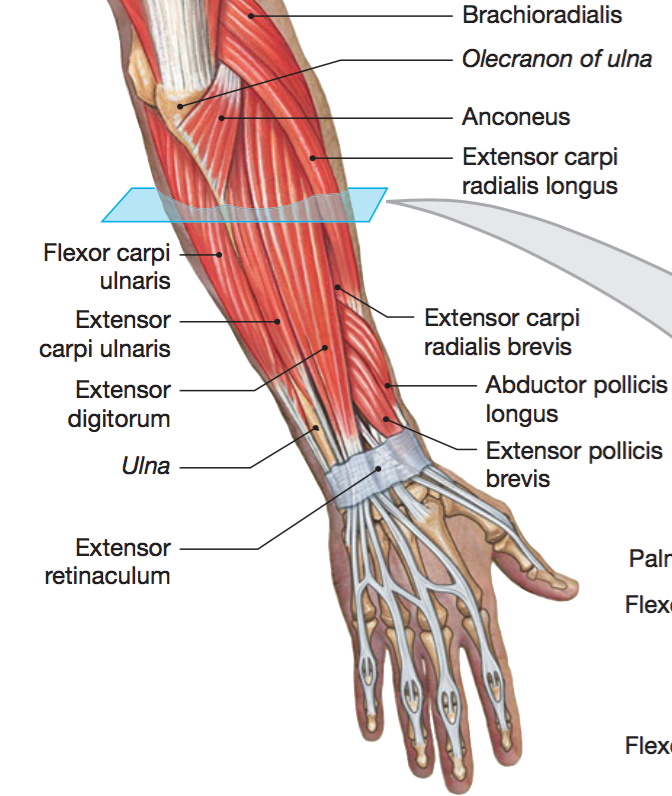
\includegraphics[width=.46\textwidth]{figures/Anatomy/posteriorSuperficial}         %\
	}                                                                    %\
	\hspace{5pt}                                                          %\
	\subcaptionbox  %<-----------------------------------------------------%\
	{                                                                       %\
		Counterclockwise 4Q operation.\newline                                 %\
		\emph{Posterior view of the middle muscle layer.\cite{martini}}                          %\
		\label{fig:postMiddle}                                     %\
	}                                                                           %\
	{                                                                            %\
		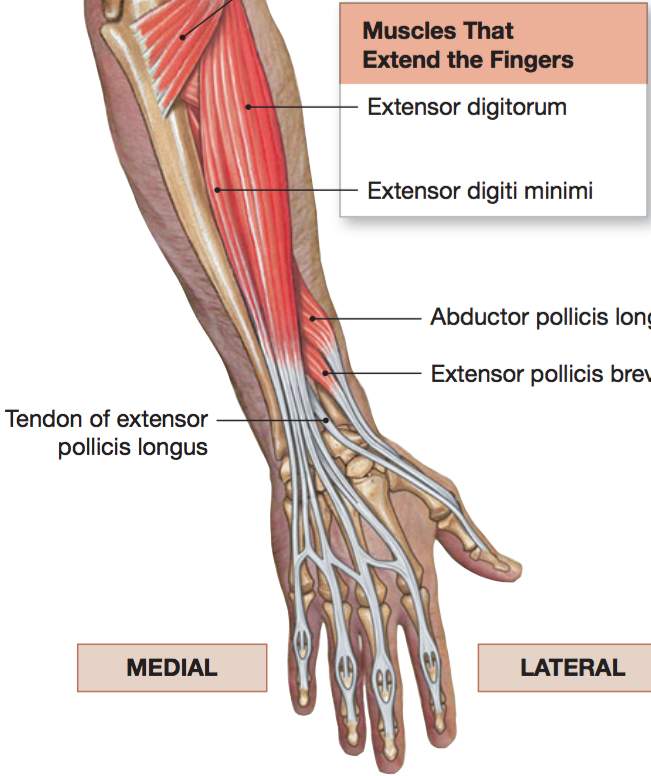
\includegraphics[width=.46\textwidth]{figures/Anatomy/posteriorMiddle}            %|
	}                                                                             %|
	\caption{Muscles and muscle layers of the forearm.}%<-%-/
	\label{fig:musclesForarm}
\end{figure}

The aim for this paper/project is to translate pronation and supination of the wrist along with extension and flexion fingers via EMG signals to control a robotic arm. Therefore, only selected muscles will be relevant to further investigate. 
Muscles involved with pronation of the wrist includes the pronator quadratus and pronator teres muscles. The pronator quadratus muscle is located near the wrist and is fixated on the distal portions of both ulna and radius, from where is forms a wide band across the gab of the two bones. The pronator teres is located near the elbow, where it originates  from the medial distal part of humerus and the medial lateral part of ulna, to reach across the anterior part of the forearm and fixate to the midlateral surface of radius. 
There is only one muscle involved in the process of supination of the forearm, the supinator. The supinator muscle sits opposite the pronator teres muscle near the elbow, where it originates from the lateral distal part of humerus and the lateral proximal part of ulna and fixate on the anterolateral surface of radius. 
These three are the only muscles responsible for pronation and supination of the forearm. Therein exists a problem in detecting viable EMG signals to properly detect pronation and supination gestures, since the muscles involved does not extend through the forearm as most other muscles in the forearm. \cite{martini}
%luckily for us both the pronator teres and supinator muscles are in the superficial muscle layer making them easily accessible for EMG detection.

Extension and flexion of the fingers include most of the muscles in the lower arm. Most of these muscles extend throughout the whole forearm as most of them originates from the lateral surfaces of humerus or the proximal portions of ulna and radius, and extends towards the wrist and fingers to fixate on the metacarpal bones in the wrist and through tendons fixate on the different phalanges bones of the fingers and thumb. See \ref{fig:wrist} and \ref{fig:wristFingers} for a detailed overview of each muscles origin, insertion and action it performs. \cite{martini}

\begin{figure}[H]
	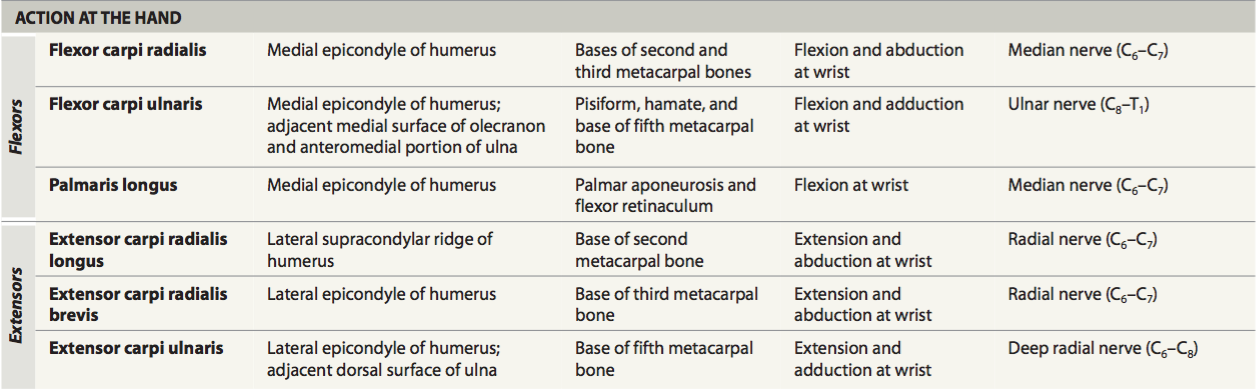
\includegraphics[width=.4\textwidth]{figures/Anatomy/wrist}  %<--but is not needed.
	\caption{Table of the muscles in the forearm involved with movements of the wrist. \cite{martini}}
	\label{fig:wrist}  %<--give the figure a label, so you can reference!
\end{figure}

\begin{figure}[H]                    
	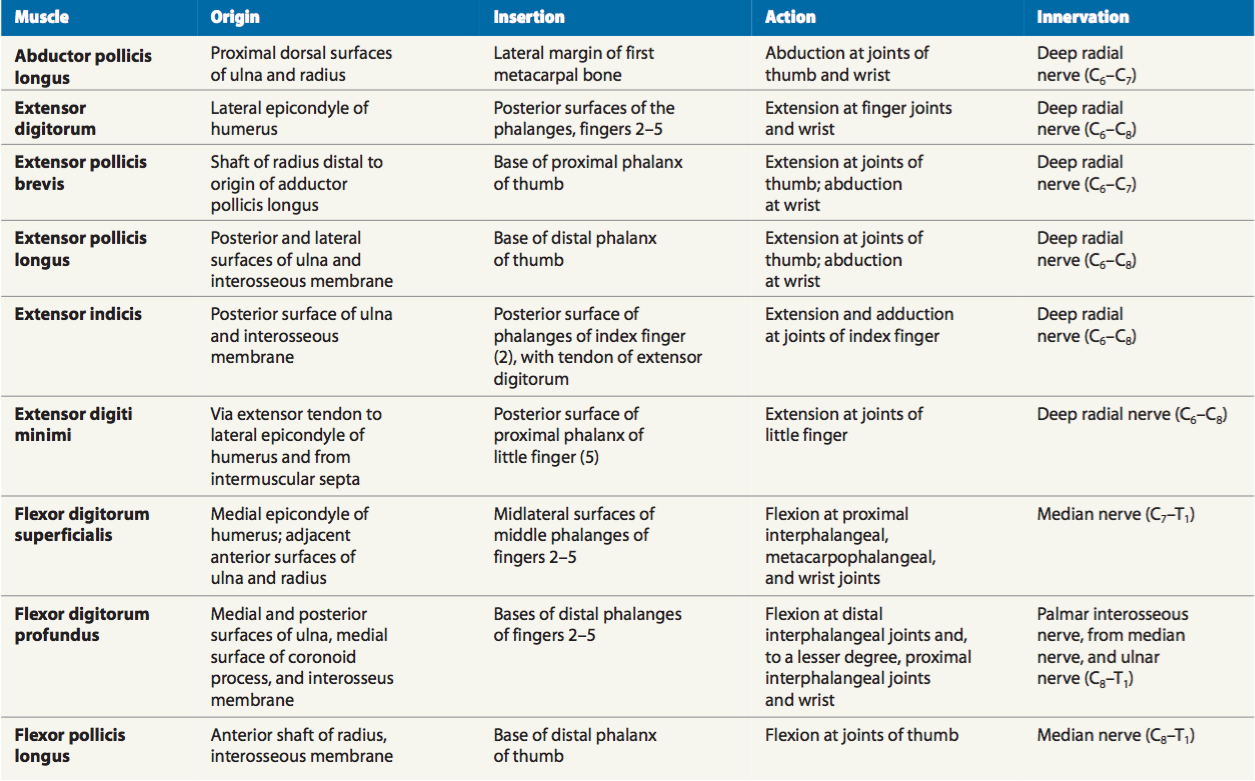
\includegraphics[width=.4\textwidth]{figures/Anatomy/wristFingers}  %<--but is not needed.
	\caption{Tabel of muscles in the forearm involved with movements of the wrist and fingers. \cite{martini}}
	\label{fig:wristFingers}  %<--give the figure a label, so you can reference!
\end{figure}



%abductor pollicis longus
%extensor pollicis longus
%extensor pollicis brevis
%extensor indicis
%supinator
%anconeus
%extensor digitorum
%extensor digiti minimi
%pronator quadratus
%flexor digitorum superficialis
%brachialis
%flexor pollicis longus
%flexor digitorum profundus
%brachioradialis
%flexor carpi ulnaris
%pronator teres
%extensor carpi ulnaris
%extensor carpi radialis brevis
%extensor carpi radialis longus
%palmaris longus
%flexor carpi radialis




%tail



